%!TEX root = ../thesis.tex
%*******************************************************************************
%****************************** Third Chapter **********************************
%*******************************************************************************
\chapter{Design and Implementation}

% **************************** Define Graphics Path **************************
\ifpdf
    \graphicspath{{Chapter3/Figs/Raster/}{Chapter3/Figs/PDF/}{Chapter3/Figs/}}
\else
    \graphicspath{{Chapter3/Figs/Vector/}{Chapter3/Figs/}}
\fi

Moving onward from our requirements, we take the first step in producing our final product. Prior to development however is the setup of our working environment, which is of importance if we are to describe the issues and choices in development, preventing or influencing what were capable of. 

\section[Development Environment]{Development Environment}
Our development setup is shown in Table \ref{tab:t1}. Evidently, we have enough hardware capabilities to meet the baseline requirements of our tools. However, this still led to issues described in later segments, including out of memory errors and erroneous execution times. Although, we did not experience all errors on our test server. 

\begin{table}
	\caption{Development Setup}
	\centering
	\label{table:good_table}
	\begin{tabular}{l l}
		\toprule
		Feature & Description  \\ 
		\midrule
		Operating System & Ubuntu 16.10 64-bit \\
		Programming Language &  Python 2.7\\
		Programming Language Tools & numpy, timeit, matplotlib\\
		Command Line Tools & dreadnaut, nauty/Traces \\
		Versioning & Github (Public Repo) \\
		RAM & 8GB DDR3 \\
		Disk & 500GB ATA SanDisk Ultra II SSD \\
		CPU & 8 x Intel Core i7-3612QM CPU @ 2.10GHz \\
		\bottomrule
	\end{tabular}
	\label{tab:t1}
\end{table}



\section[Architecture]{Architecture}
Our system setup separates development and experiment stages of our program. We first created our package on a laptop computer, which would regularly update experiments, data and code through SSH, FTP and GitHub respectively. Once experiments were completed, we would save these results to our repository and then generate plots. This was to esnure that the python process in action would remain undisturbed by any other system process. Both systems used a form of Linux, and the experiment server was hoster on Digital Ocean, which allowed us to change system resources as required. This is important to note as we frequently had to do this.
\par
\begin{figure}[htbp!]
	\begin{center}
		\leavevmode
		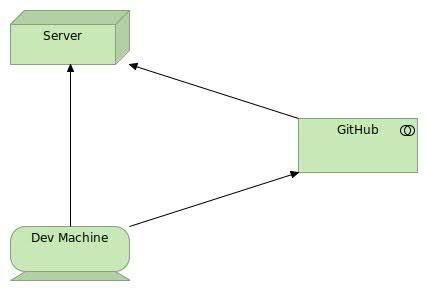
\includegraphics[height=50mm]{Figs/architecture.jpg}
	\end{center}
	\caption{System Architecture}
	\label{fig:one}
\end{figure}
\begin{figure}[htbp!]
	\begin{center}
		\leavevmode
		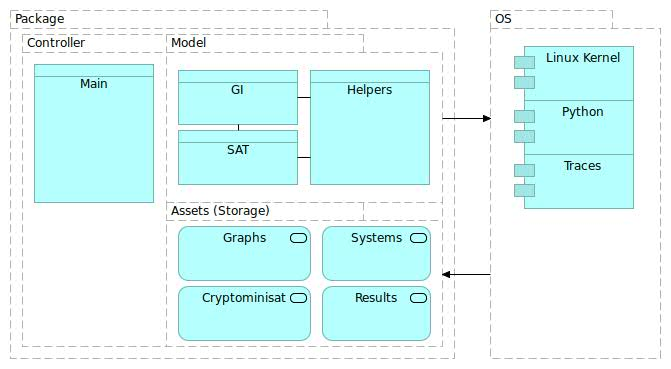
\includegraphics[height=50mm]{Figs/implementation-architecture.jpg}
	\end{center}
	\caption{Software Architecture}
	\label{fig:one}
\end{figure}

\section{Algorithms}
We two major steps in our program: locating our desired systems, and then converting them to our construction. With the added stages of separating graphs into packages which varied in complexity, and then executing these graphs to find execution times, we have a total of four key steps. The following diagram depicts our workflow:

\begin{figure}[h]
	\centering
	\begin{tikzpicture}[
	node distance = 5mm and 7mm,
	start chain = going right,
	alg/.style = {draw, align=center, font=\linespread{0.8}\selectfont}
	]
	\begin{scope}[every node/.append style={on chain, join=by -Stealth}]
	\node (n1) [alg] {Find \\ systems};
	\node (n2) [alg]  {Convert \\ to graphs};
	\node (n3) [alg]  {Seperate \\ into packages};
	\node (n4) [alg] {Benchmark \\ tests};
	\end{scope}
	\end{tikzpicture}
	\caption{Typical workflow}
	
	
\end{figure}
Each stage has its own form of elaborate checks and logic. Here we will describe each part does, how it is integrated into our architecture and notable pieces of logic. Note that this is the most basic usage of our software, and additional features and options are mentioned later. We will only describe the first two parts here, and the second parts in the Evaluation, as the following steps were a result of findings. 

\subsection{Timing}
Times were monitored using pythons Timeit library. If a timeout was specified, and exception would be thrown and han[ht]dled appropriately. Runs which required the uses of system calls, such as dreadnaut and Traces, would be called using the Process Handler. One would record the time before and after the call was made. Granted this does not give the very accurate times, but was satisfactory enough to gauge the general idea. We assumed that making the system call would only add sub second times to overall execution, which results in no large changes in the execution of large graphs, which executed for multiple minutes. 
\newpage
\subsection[Systems Search]{Systems Search}
Given values max\_n	and max\_m, the maximum number of clauses and literals respectively, we search for systems in the following manner (see algorithm for details): let $n=m=4$; iterate over the set $N=\{n, n+step,..,max\_n\}$; for each $n \in N$, iterate over the set $M=\{m, m+step,..,max\_m\}$; for these values of $n$ and $m$, generate a random system of equations from a pool of $n$ literals, that is $\{1,2,..,n\}$ with $m$ clauses; validate this system for unique satisfiability and k-local consistency; if it is valid, then store this system. See Algorithm \ref{alg:a1}.
\par
There are, of course, may checks not mentioned, however, we take this as the simplest form of generating a range of systems, over the Cartesian product of $N$ and $M$, where $n \leq m$. Thereby ranging from the line of satisfiability, $n=m$, to some $n=max_n$ and $m=max_m$

\begin{algorithm}[htbp!]
\SetAlgoNoLine
\KwIn{Integers $min\_n$, $min\_m$, $max\_n$, $max\_m$, $step$, $max\_tries$.}
\KwOut{A set of uniquely satisfiable and k-locally consistent XOR-Formulas.}
$systems = \{\}$\;

\Repeat{$min\_n$ == $max\_n$}{
	$tries = 0$\;
	
	\Repeat{$min\_m$ == $max\_m$}{
		\If{$tries == max\_tries$}{
			$tries = 0$\;
			$min\_m += step$\;
			skip this iteration\;
		}
		
		$system$ = Generate random system($min\_n, min\_m$)\; 
		\eIf{system is uniquely satisfiable and k-locally consistent($system$)}{
			$systems$ add $system$\;
			$tries = 0$ \;
			$min\_m +=step$\;
		}{
		$tries += 1$\;
	}	
}
$min\_n += step$\;
}

return $systems$
\caption{Fundamental Search: Finding uniquely satisfiable and k-locally consistent systems}
\label{alg:a1}
\end{algorithm}

\newpage
\subsection{Constructing Graphs}
In transforming eligible systems into our final construction, we must first ensure that the graphical representation of our XOR-Formula contains no automorphisms. This is determined by Traces, and is fairly easy to compute. Once this is decided, them we we apply the multipede structure on our graph, resulting in the final product. Recall in the background segment we label the preliminary and final graphs $G_A$ and $G_B$ respectively. See Algorithm \ref{alg:a2}.
\par
$G_A$ is trivial to construct into its graphical representation, whereas $G_B$ requires only slightly more logic. We used numpy matrices to construct adjacency matrices from a system, which worked sufficiently well for large systems. 
\begin{algorithm}[htbp!]
		\SetAlgoNoLine
		\KwIn{Integers $n$, $m$.}
		\KwOut{A set of random 3 literal clauses}
		$pool = \{1,2,..,n\}$\;
		$system=\{\}$\;
		$tries=3$\;
		$index=0$\;
		
		\Repeat{$index$ == $m$}{
			\If{$tries==0$}{
				return $False$\;
			}
			$clause$ = random 3 literals from $pool$\;
			\eIf{$clause \in system$}{
				$tries-=1$\;
			}{
			$system$ add $clause$\;
			$index+=1$\;
		}
	}
	
	return $systems$
	\caption{Generate random system}
	\label{alg:a2}
\end{algorithm}



\newpage
\section{Parameter Settings}
During implementation, many constants and variables were assigned values in response to issues. These hard coded values are of importance when we discuss results. For the meantime, we will define them here so that they can easily be identified. See the following table for descriptions.

\begin{table}[h]
	\centering
	\label{tab:parm}
	\begin{tabular}{p{2cm}| p{11cm}}
		\toprule
		Parameter & Description \\
		\midrule
		Step & Searching for systems requires some iterator over n and m. This increments m by some value. \\ \hline
		Limit &  We may want to find this number of systems from a given m. Useful if we want to find the smallest ratios. \\ \hline
		Tries & Generating random systems has two problems: 1, we include the same clause twice from a pool of literals. 2, The system may not match our criteria Therefore, we try this many times before moving on.\\ \hline
		Timeout & dreadnaut, nauty/Traces \\ \hline
		Upper bound and lower bound & Suppose we wanted to search along the threshold of satisfiability. we would set this value to 1. This describe the upper and lower bound of n = u * m, for some u.\\ \hline
		Defaults & n=m \\
		\bottomrule
	\end{tabular}
	\caption{Search parameters}
\end{table}
\newpage
\section{Development Issues}
Faults are inevitable in ever undertaking, and ours are reported in this segment.
\par
We noticed during execution strange behaviour from Traces and the operating system. This is notable  since these issues may effect our report of results, although, these issues may be uncommon and spurious. 

\subsection{Python OOM}
Python processed tended to crash after short periods of time on the experiment server. This required swap space to be allocated as RAM was not satisfactory. Attempts were made without having to include swap space, the caveats being access to secondary memory should be averted. However, larger implementations which included a 2 CPU machines with 2gb RAM still was not satisfactory. Therefore, swap space must be included on small installations. 

\subsection{Traces OOM and Indefinite Execution}
Traces was expected to halt when instances became too large to process. Luckily, our construction was below this threshold for small instances that mattered. However, at node sizes roughly at 6000, Traces began to fall short at seemingly random times. Occasionally, Traces would run one graph for an indefinite period of time (which had to be manually cancelled), and for another run, ran for a few hours. Given that we had the instances we needed, this issue was not explored, and may have only been an operating system issue, since 20gb swap space had to be allocated to permit for larger instances.
\par
For some instances, even at the relatively small end of our graphs, which consisted of a manageable number of nodes, say 4000, Traces would crash unexpectedly after multiple hours. The details of these instances were not recorded, however for relatively small values of our graphs, graphs which executed for numerous hours, say n=500, Traces would fail. It is unknown whether this due to hardware insufficiencies. Therefore, for instances which timeout, where no timeout is defined - this describes a system error of some sort. One such example is the tnn(2) graph, whose similar graph tnn(1), would run for multiple days, causing strange CPU behaviour. There is a picture of this issue displayed in appendix. The cause is unknown, a snapshot of the development server is also placed in the appendix to reproduce problems. Hence, some instances which timed out, may have in fact fell under this bug. It is quite possible that instances became too complex at a point, which required more swap space than allocated. However, this is only a speculation.

\section{Additional Features}
Given that there is more than one way to program our logic, multiple strategies were used to generate our desired construction. Here we define additional methods utilised and features that extended beyond our requirements and design. They may be of importance in future applications.

\subsection{Alternative XOR-Formula Generation}
Our algorithm to generate desired systems picks three random literals and adds these to a set of clauses. However, for some values of n and m, a system cannot be located. We know that there exists a suitable system for these values, but cant be selected at random due to the large permutation of n. For small values of n and m, we believed that all combinations could be held in memory and systematically tested, rather than being generated at random. Hence, a recursive search is provided to find all combinations to be tested. However, in implementation, this could not be used even for small values of n and m due to running times. Nonetheless, this feature may be of importance when time is not an issue, and a set of desired systems are required for given values.

\subsection{Updating Slow Systems}
Since we determine k-local consistency by checking if one system executes faster with Gauss-On versus Gauss-Off, it can be problematic to determine if a system is suitably slow. Small systems execute very quickly, and differ into two runs by only sub second values. These sub second difference could be mistaken for fluctuations in system performance, rather actual operating time (since we are measuring time not by process execution time, but start and end times). Here we have two solutions to mitigate this error.
\par
The first solution is to use some parameter, say \emph{minimal\_difference}, to provide a lower bound on the value required for a k-locally consistent system. However, this may be too large for small systems to register or too small to attain difficult instances. The second option is to solve this problem by repeating runs. We save those systems which have the largest difference in a separate directory, and replace these systems when comparing differences. If a newly found system is slower, that is it has a larger positive difference than the stored one, then we replace the stored one. This way, by using many iterations, we can generate a set of systems which have the largest differences to date. We are able to filter out those instances with exceptionally slow times. These graphs will be the most difficult found, and thus, the ideal type to construct to use in benchmarking. We prove this experimentally.

\subsection{Advanced Search}
Considering that we must check if a suitable system gives rise to a graph with no non-trivial automorphism, we can combine this check when searching for systems. In addition to updating strongly k-systems, we have the tools to search for the ideal graph.
\par
If we convert the system to a graph and check for automorphisms on the fly, that is, whilst searching and validating systems, we eliminate the need to build up a database of suitable systems up to the point of automorphisms, at the cost of running time. Thus, the search can be computationally heavy, but we ensure that every proceeding search is better than the last. There are parameters defined enabling us to use this extended validation check.

\subsection{Optimised Search}
Numerous parameters are available to speed up searching. Here we briefly describe how they can be used.
\par
The upper bound and lower bound variables search for a given region of n and m. For example, if we wanted to search for systems along the line of satisfiability, we would set both values to 1. This would ensure we get the most difficult instances possible, but results in longer execution time due to failed tries (see Section 5). Moreover, we can check along n=2m or between n=m and n=2m, and so forth.
\par
Similar to the upper bound and lower bound variables, the limit variable permits us to search for a given number of systems for a given n. That is, move up n by step if we have found $limit$ systems. This is important when we consider the next paragraph.
\par
Efficient search variable checks that we solve the following optimisation problem. If we begin by searching along the line n=m, for large n, and no such system was found up until n=2m, then it is unlikely that the following iteration $n=n+step$ will find a system between n=m and n=2m. Thus, efficient search remembers the last good m value. Thereby eliminating the need to make redundant checks. This is useful, for suppose we set limit=1, lower-bound = upper-bound = 1, tries = 1000, $update\_strongly\_k = true$, then we could efficiently find systems close the the threshold of satisfiability. A number of these example searches are provided in the appendix. 
 \newpage
\subsection{Extending Traces Benchmarks}
To permit us to see how large we could potentially make out construction, numerous random graphs provided by Traces were extended. Graphs with edge probability 1/2, 1/10 and sqrt(n) were constructed using programs provided by the nauty/Traces suite: genrang (to build) and showg (to convert .g6 to .dre). Instances ranged from 5 to 30,000 nodes, and were executed successfully.
